% !TeX spellcheck = zh_CN
% !BIB program = bibtex
\documentclass[aps,pre,12pt,preprint,%
	onecolumn,showpacs,showkeys,nofootinbib]{revtex4-1}
%UnlimitedFonts
	\def\hmmax{0}
	\def\bmmax{0}
%SVG
	\usepackage{svg}
%Tables
	\usepackage{array,booktabs,tabularx,multirow}
	\newcolumntype{C}[1]{>{\hsize=#1\hsize%
		\centering\arraybackslash}X}
%Math&Fonts
	\let\latexointop\ointop
	\usepackage{mathtools,amssymb,bm % basics
		,physics,siunitx,slashed % physics
		,esint,nicefrac,extarrows,mathrsfs % more symbols
		,calligra,romannum,dsfont,fourier-orns % nice fonts
		,eqnarray,resizegather,empheq % more envs
		,relsize,stackengine % utils
	}
%	\usepackage{amsthm}
	\usepackage[scr=esstix]{mathalfa}
	\usepackage[only,sslash]{stmaryrd}
	%DisplaySetup
	\newcommand*\bbox[1]{\fbox{\hspace{1em}\addstackgap[5pt]{#1}\hspace{1em}}}
	\empheqset{box=\bbox}
	\mathtoolsset{showonlyrefs}
%Utils
	%Legacy \oint
	\let\ointop\undefined
	\let\ointop\latexointop
	%Calligra
	\DeclareMathAlphabet{\mathcalligra}{T1}{calligra}{m}{n}
	\DeclareFontShape{T1}{calligra}{m}{n}{<->s*[2.2]callig15}{}
	%CosmeticTweaks
	\newcommand\inlineeqno{\stepcounter{equation}\ (\theequation)}
	\newcommand\scalemath[2]{\scalebox{#1}{\mbox{\ensuremath{\displaystyle #2}}}}
	\newcommand\raisemath[2]{\raisebox{#1\depth}{${#2}$}}
	\newfontfamily\signature{Vladimir Script}
	\newcommand{\newparagraph}{\pagebreak[3]
		\noindent\hfil%
		\raisebox{-4pt}[10pt][10pt]{\leafright~\qquad~\leafleft}%
		\par\nopagebreak%
	}
%CustomCmds
	%Brackets
	\DeclarePairedDelimiter\ave{\langle}{\rangle}
	\DeclarePairedDelimiterX\inprod[2]{\langle}{\rangle}{#1,#2}
	%Basics
	\newcommand{\mbb}[1]{\mathbb{#1}}
	\newcommand{\mrm}[1]{\mathrm{#1}}
	\newcommand{\mcal}[1]{\mathcal{#1}}
	\newcommand{\mscr}[1]{\mathscr{#1}}
	\newcommand{\tup}[1]{\textup{#1}}
	\newcommand{\mop}[1]{\operatorname{#1}}
	%Extras
	\newcommand{\scriptr}{\mathcalligra{r}\,}
	\newcommand{\rvector}{\pmb{\mathcalligra{r}}\,}
	\newcommand{\hodgedual}{\operatorname{\star}}
	\newcommand{\dual}{\ \xlongleftrightarrow{\ \textrm{dual}\ }\ }
	\newcommand{\idty}{\mathds{1}}
	\newcommand{\proj}[1]{\operatorname{%
		proj_{\mathit{#1}}}}
	\newcommand{\propsim}{\mathbin{\ensurestackMath{
		\stackunder[2pt]{\propto}{\sim}
	}}}
	\newcommand{\textbox}[1]{\fbox{#1}}
	\newcommand{\pdd}[1]{\operatorname{\partial_{\mathnormal{#1}}}}
	\newcommand{\cdd}{\operatorname{D}\!}
	\newcommand{\cdv}[1]{\operatorname{%
		\nabla_{\!\mathit{#1}\!}}}
	\newcommand{\ldv}[1]{\operatorname{%
		\mcal{L}_{\!\mathit{#1}\!}}}
	\newcommand{\ric}[1]{\operatorname{%
		Ric}\!\pqty{#1}}
%Hacks
	% physics.sty <texmf-dist/tex/latex/physics/>
	% USER: more spacing around Dirac's middle vert
	\newcommand{\xmiddle}[1]{\mspace{1mu}\middle#1\mspace{1mu}}
	\DeclareDocumentCommand\innerproduct{ s m g }
	{ % Inner product
		\IfBooleanTF{#1}
		{ % No resize
			\IfNoValueTF{#3}
			{\vphantom{#2}\left\langle\smash{#2}\xmiddle\vert\smash{#2}\right\rangle}
			{\vphantom{#2#3}\left\langle\smash{#2}\xmiddle\vert\smash{#3}\right\rangle}
		}
		{ % Auto resize
			\IfNoValueTF{#3}
			{\left\langle{#2}\xmiddle\vert{#2}\right\rangle}
			{\left\langle{#2}\xmiddle\vert{#3}\right\rangle}
		}
	}

%Miscellaneous
%	\newcommand{\tabindent}{\hspace{2em}}
	\newcommand{\naItl}{\tup{NaI\,(Tl)}}
	\newcommand{\perc}[1]{\SI{#1}{\percent}}
	\newcommand{\csAtom}{${}^{137}\mrm{Cs}$}
	\newcommand{\coAtom}{${}^{60}\mrm{Co}$}
	\newcommand{\rayleighNumber}{\mrm{Ra}}
\begin{document}
%Basic Data
	\title{%
	\texstringonly{\hfil\\[2\baselineskip]}
	\sf\LARGE%
		利用磁光克尔效应测定样品的磁滞回线%
	\texstringonly{\vspace{3ex}}}
	\author{\fangsong\large%
		Bryan%
	\vspace{2mm}}
	\affiliation{\it%
		北京大学物理学院~~学号:\normalfont 1500066666\,}
	\date{\today}
	\keywords{
		磁光克尔效应\quad 光弹调制\quad 锁相放大\quad 克尔磁滞回线
	}
	\email{masked_email_please_contact@github.com}

\begin{abstract}
\vspace{10mm}
\begin{spacing}{1.5}\normalsize
\setlength{\parskip}{.3\baselineskip}
%	200—300字,
%	说明用什么方法做了什么事,
%	由此得到什么结果和结论,
%	有何意义.
%	不用缩略词,不用第一人称.
%%%%%%%%%%%%%%%%%%%%%%%%%%%%%%%%
	本实验观察了不同外磁场下铁磁样品表面反射光的偏振变化,获得了样品的磁滞回线,由此验证了磁光克尔效应。
	
	具体而言,实验中利用光弹调制器和锁相放大器分析了极克尔效应的出射光,以微机自动化的方法对微小的克尔转角和克尔椭偏率与磁场的关系进行了精确测量,由此获得了克尔磁滞回线,并测得了样品的饱和克尔转角与矫顽力。
\end{spacing}
\end{abstract}

\maketitle
\thispagestyle{titlepagestyle}

%%  课程实验报告应假定读者既不是已知全部实验细节的指导教师,也不是缺少专业知识的公众,而是同领域的实验研究者,或审稿人. 不能要求读者要在读过课程讲义后才能读懂课程实验报告.
%%  凡不是自己独立思考得到的内容都应该引参考文献. 不能大段引用同一参考文献. 对复杂问题,应该优先考虑引用参考文献得到结果. 对简单一些的问题才鼓励独立思考.
\section{引言}
%%	研究论文引言一般包含以下内容:
%%	(1)所研究领域背景和现状;
%%	(2)有待研究的问题;
%%	(3)本研究的目的、主要内容和结果;
%%	(4)结果的意义.\par
%%	在写实验报告的引言时,同学可以假想自己是第一个做类似研究的人.\par
%%	引言一定要切合报告正文,不能漫无目的地介绍背景. 要快速地将读者引导到报告主题上,并作较深入的讨论.\par
%%	引言篇幅可以在较大范围内变化,但最长不应超过报告文字篇幅的1/3.\par
%%	引言撰写可以参考实验讲义,可以复述,但不能复制讲义上的任何一句话.\par
%%%%%%%%%%%%%%%%%%%%%%%%%%%%%%%
\vspace{-.5\baselineskip}
	1877年,克尔(J. Kerr)发现平面偏振光从光洁磁极表面反射时, 偏振面会发生微小偏转 \cite{kerr1877xliii}, 此即磁光克尔效应。克尔的研究本身受到了法拉第效应的启发;1845年法拉第(M. Faraday)发现,平面偏振光穿过在光的传播方向加有磁场的玻璃时,偏振面会转过一个角度 \cite{faraday1933faraday}, 此即法拉第效应。
	
	上述两个效应均为磁光(magneto-optic)效应,体现了物质磁化状态对其光学性质的影响。它们的物理根源实际上是一致的;经典图像下,它们均源于洛伦茨力对电子运动的影响 \cite{textbook}. 更进一步,1896年塞曼(P. Zeeman)指出 \cite{zeeman1896ueber}, 磁场中的光源谱线会发生分裂,得到若干偏振化的谱线;正常塞曼效应实际上也可由上述经典极值解释,只不过某些情况下须考虑电子自旋的影响,此即反常塞曼效应 \cite{sakurai2014modern}. 
	
	磁光效应具有广泛的应用;如利用磁光克尔效应改进存储介质一度是研究的热点 \cite{textbook}. 本实验即通过观察极入射线偏光的反射偏振随外磁场的变化,以验证磁光克尔效应,并了解其背后的物理机制。
\vspace{-.5\baselineskip}
\section{理论}
\vspace{-.5\baselineskip}
%\setlength{\jot}{0pt}
	经典图像下,介质的介电张量$\epsilon$可由受迫振子模型描述;引入磁场后,只须附加考虑洛伦茨力的影响。对沿磁场方向传播的左旋圆偏光,相应地有 \cite{textbook}: 
	\begin{equation}
		n^2_+(\omega) = 1 + \frac{Ne^2}{m\epsilon_0}\,
			\frac{1}{
				(\omega_0 + \omega_L)^2 - \omega^2 - i\gamma\omega
			},\quad
		\omega_L = \frac{e}{2m}\,B
	\end{equation}
	其中$m$: 电子质量,$e$: 电荷单位,$N$: 单位体积振子密度,$\epsilon_0$: 真空介电常量,$\gamma$: 阻尼系数,$\omega_0$: 固有频率,而$\omega_L$正是电子轨道磁矩在外磁场中的经典进动频率——Larmor进动频率。若考虑右旋圆偏光,则$\omega_L \mapsto -\omega_L$. 
	
	直观上,磁场的存在改变了圆偏光下电子回旋的固有频率。对于磁性物质而言,此时电子的自旋不可忽略,故还须考虑量子力学中自旋轨道耦合的影响,详细分析参见 \cite{textbook}. 
\clearpage
	
	综上,磁场导致了各向异性的介电张量$\epsilon$, 且其对应的本征态为左、右旋圆偏光。本实验仅考虑极入射极克尔效应,此时磁场、入射光线均垂直与样品表面,系统具有旋转对称性;据Fresnel公式,此时反射率:
	\begin{equation}
		r_\pm = \frac{1 - n_\pm}{1 + n_\pm}
	\end{equation}
	$n_\pm$分别为左、右旋圆偏光的折射率,由此导致入射的线偏光(左、右旋圆偏光的叠加态)反射后称为长轴略微偏离入射偏振面的椭偏光,偏离程度可由复克尔转角$\tilde{\theta} = \theta + i\epsilon$加以刻画,其中$\theta$为实转角,而$\epsilon$所得椭偏光的克尔椭偏率(椭圆短、长轴之比)。有:
	\begin{equation}
		\tan\tilde{\theta}
		= \frac{i\,\frac{r_+ - r_-}{2}}{\frac{r_+ + r_-}{2}}
		= i\,\frac{r_+ - r_-}{r_+ + r_-}
	\end{equation}
	
	一般来说,$\tilde{\theta}$是十分微小的,其精确测量存在一定的技术困难;本实验中其测定通过光弹调制与锁相放大实现。其中,光弹调制器可使特定方向的线偏光附加上随时间振荡的相位$\delta(t) = \delta_0\sin\omega t$, 配合后端的 \ang{45} 角检偏器,可使出射光强的谐波分量承载上不同方向的偏振信息;进一步由锁相放大提取谐波分量强度,即可得到$\tilde{\theta}$. 
	
	\cite{textbook} 中分析表明,若取光弹调制振幅$\delta_0\simeq 2.405$, 即为零阶Bessel函数的零点$J_0(\delta_0) = 0$, 则恰有:
	\begin{equation}
		\theta = \frac{\sqrt{2}V_{2\omega}}{4V_0 J_2(\delta_0)}
		\propto \frac{V_{2\omega}}{J_2(\delta_0)},\quad
		\epsilon = - \frac{\sqrt{2}V_{\omega}}{4V_0 J_1(\delta_0)}
		\propto - \frac{V_{\omega}}{J_1(\delta_0)}
	\label{eq:signalHarmonics}
	\end{equation}
	这里$V_0,V_\omega,V_{2\omega}$分别为锁相放大得到的直流、一次、二次谐波分量。
%\restorejot
%%%%%%%%%%%%%%%%%%%%%
\clearpage
\section{实验装置}
%\vspace{-.5\baselineskip}
	实验装置如图 \ref{fig:apparatus} 所示,入射激光经起偏器的线偏光,近似垂直入射样品表面;出射光经光弹调制、检偏、光电探测转化为电信号,进而由锁相放大提取出谐波分量,输入计算机。外磁场同样由计算机控制,通过调整励磁电流以调整外磁场$B$的大小,利用高斯计监测并反馈调节所需磁场。
	
	\begin{figure}[!ht]
		\centering
%		\hspace{-.1\linewidth}%
		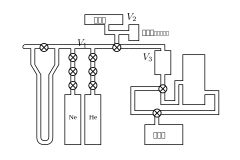
\includegraphics[width=.85\linewidth]{img/apparatus.png}
		\par\vspace{.5\baselineskip}
		\caption[磁光克尔效应实验装置]{%
			磁光克尔效应实验装置示意图,参见 \cite{textbook}. %
		}
		\label{fig:apparatus}
%		\vspace{-1\baselineskip}
	\end{figure}
	
	实验前首先调整好相应仪器的推荐工作参量,并调节光路与偏振片方向以满足要求。此外,由于光电转换、放大过程引入的未知系数,须对 \eqref{eq:signalHarmonics} 式中的比例系数进行定标,这通过改变入射偏振方向、测定小角近似下$\tilde{\theta}$的线性变化实现。
\section{结果与分析}
%	实验结果应尽量以图表的形式给出. 每一个图表都应该是完整的,即阅读图表时可以不必依赖正文.\par
%	依自己意愿,实验结果和对结果的分析讨论既可分为两节也可合在一节.\par
%
%	每个图一般包含:图名、轴名、轴、刻度、标尺、数据点、曲线、图例、标注和图注等部分. 应尽量让读者不看正文就能基本理解图的含意.\par
%	逐点测量得到的函数关系要同时用表格和图给出. 需要作比较的多条曲线要画在同一图上.\par
%	为避免读者在图表和正文间反复跳跃阅读,在正文中也要对图表作必要的说明.\par
%
%	对于预料之外的实验结果,必须首先小心证明其可靠性.读者只有在相信你的实验结果时才愿意花时间看你的分析.\par
%	必须用文字归纳整理出正式的实验结果或结论.可信的实验结果是课程报告最重要的内容.作为一个实验物理工作者,分析解释出错并不丢脸,实验结果不被采信则是致命的.\par
%	教学实验的结论往往是预先知道的. 所以,教师更关心的是你的说理过程. 一般说来,单由课内实验的结果不足以能得到明确的结论. 此时,你可以引用他人的研究结果来帮助帮助自己的论证,但必须注明出处. \par
%	确实不能得到明确结论时,可以给出几种可能结论并指出可以再做哪些实验来帮助作进一步的判断.\par
%	总之,分析讨论部分要做到: 论据要valid,论证要reasonable,结论要convincing.\par
%%%%%%%%%%%%%%%%%%%%%%%%%%%%%%
%\vspace{-1\baselineskip}
%\FloatBarrier
	首先进行$\tilde{\theta}$的定标,这可通过计算机半自动地实现;记起偏器刻度$\theta_0$, 相应地测得克尔转角$\tilde{\theta}$, 如图 \ref{fig:calibration} 所示,可见二者线性相关,计算机定标得系数$\sim \SI{7.3125}{\deg^{-1}}$. 在此基础上,测定$\theta_0 \simeq \ang{2.5}$时的克尔转角与椭偏率,结果如图 \ref{fig:sampleData}. 
\clearpage
	
	\begin{figure}[!ht]
		\centering\small
		\includegraphics[width=.6\linewidth]{img/calibrationPlot.pdf}
		\hspace{2em}
		\caption[克尔转角的系数定标]{克尔转角的系数定标,其中$\theta_0$为起偏器刻度,相应地测得克尔转角$\tilde{\theta}$. }
		\label{fig:calibration}
	\end{figure}
	
	\begin{figure}[!ht]
		\centering\small
		\newcommand{\figheight}{.28\linewidth}
		\includegraphics[height=\figheight]{data/plots/sampleTheta.pdf}\ 
		\includegraphics[height=\figheight]{data/plots/sampleEpsilon.pdf}
		\hspace{1.5em}
		\caption[$\theta_0 = \ang{2.5}$时克尔转角及椭偏率随磁场的变化]{
			$\theta_0 = \ang{2.5}$时克尔转角$\theta$及椭偏率$\epsilon$随磁场的变化。实测克尔转角本为左图的反相状态(即$-\theta$),这里将其乘以$(-1)$而化为了通常的磁滞回线形态。
		}
		\label{fig:sampleData}
	\end{figure}
	
	由图可见,克尔椭偏率的变化较为病态,没有明显的规律;这大概是源于光线在通过光弹调制晶体时的反射、干涉现象,这一过程可能影响一次谐波分量$V_\omega$的值,进而影响$\epsilon$的测定,如 \eqref{eq:signalHarmonics} 所示。故此后我们只关注克尔转角$\theta$的取值。
	
	对于克尔转角,这里我们观察到了明显的磁滞效应,这是由于采用了铁磁样品的缘故。实验中小范围内改变起偏器夹角$\theta_0$, 多次绘制克尔磁滞回线,如图 \ref{fig:hysteresis} 所示;可见磁滞回线的形态无显著变化,而其$\theta$位置随$\theta_0$近似线性地平移,这与图 \ref{fig:calibration} 所示的线性关系一致。
	
	\begin{figure}[!ht]
		\centering\small
		\includegraphics[width=.75\linewidth]{data/plots/hysteresisCurves.pdf}
		\hspace{3em}
		\caption[不同入射偏振时的克尔磁滞回线]{
			不同入射偏振时的克尔磁滞回线,这里$\theta_0$为起偏器刻度。
		}
		\label{fig:hysteresis}
	\end{figure}
	
	为测定饱和克尔转角和铁磁样品的矫顽力,在$\theta_0 = \ang{3}$时对磁滞回线进行密集取样,即减小磁场$B$的变化步长,结果如图 \ref{fig:hysteresisDetailed} 所示;可见$\abs{B} > \SI{500}{\milli\tesla}$时基本实现了饱和磁化,对这些数据进行平均,得到饱和克尔转角$\theta_{\max} \simeq \ang{.301}$. 
	
	矫顽力则由$\theta$校正后的曲线零点给出,插值给出的零点分别为$213.676,-214.965$, 单位$\si{\milli\tesla}$, 可见曲线并非十分对称,这可能源自测量误差或涨落;左右平均,给出矫顽力$B_0\simeq \SI{214}{\milli\tesla}$. 
	
	\begin{figure}[!ht]
		\centering\small
		\includegraphics[width=.75\linewidth]{data/plots/hysteresisDetails.pdf}
		\hspace{3em}
		\caption[$\theta_0 = \ang{3}$时的克尔磁滞回线]{
			起偏器刻度$\theta_0 = \ang{3}$时的克尔磁滞回线,已通过零点修正\\
			($\simeq -1.51806$的平移)使$\theta$的范围关于零点$\theta = 0$上下对称。
		}
		\label{fig:hysteresisDetailed}
	\end{figure}
\section{结论}
\vspace{-.5\baselineskip}
%%%	首先要给出实验结果,然后再给出由实验结果分析得到的结果和结论。此部分给出的内容要比摘要中的全面,用词要更准确。\par
%%%%%%%%%%%%%%%%%%%%%%%%%%%%%%%	
	本实验通过半自动化的现代手段测定了铁磁样品的克尔磁滞回线,由此验证了磁光克尔效应,并进一步测定了样品的饱和克尔转角$\theta_{\max} \simeq \ang{.301}$及矫顽力$B_0\simeq \SI{214}{\milli\tesla}$. 
\raggedbottom
\section{致谢}
\vspace{-.3\baselineskip}
%	此部分感谢同组人...和对实验和报告有帮助的人。
%%%%%%%%%%%%%%%%%%%%%%%%%%%%%%
	感谢周路群老师的细致指导,尤其是老师关于实验基本原理的启发对本人带来了很大帮助;感谢合作者余忠德同学的工作和帮助。
%	感谢 \TeX\, - \LaTeX\, Stack Exchange\footnote{%
%		\url{https://tex.stackexchange.com/}
%	}, 助我解决了众多排版问题。
\vspace{.3\baselineskip}

\setlength{\bibsep}{1ex}
\linespread{1.}\selectfont
\bibliographystyle{../BibStyle/gbt-7714-2015-numerical}
%\bibliographystyle{apsrev4-1}
\bibliography{../BibStyle/Textbook,bib/Ref}
\clearpage
\linespread{1.5}\selectfont
\end{document}